\chapter{Experimental Setup}
\label{chapterlabel4}

\section{Collaboration with BBC News Lab}
\section{Dataset}
News is the contemporary witnesses of the world and tremendous number of news are generated every day. According to Chartbeat\footnote{http://www.slideshare.net/chartbeat/mockup-infographicv4-27900399}, over 92,000 news are posted to the web every 24 hours which is nearly impossible for human processing and tagging. Therefore BBC News Lab has launched the project \footnote{http://bbcnewslabs.co.uk/projects/topic-modeling/} collaborating with UCL to try to automatically nail down "What is this news about?" in a few words. 
The news stream is provided by BBC news using \textit{The Juicer} which is a news aggregation and content extraction API \footnote{http://bbcnewslabs.co.uk/projects/juicer/}. In order to capture the dynamic nature of the news we have crawed the BBC news in a long time range - from January 1st, 2016 to May 31st, 2016 - for the experiment's purpose.
The corpus has collected all 36162 news published by BBC covering the period of 152 days. For the purpose of experimenting dynamic author-topic model we assume the news in a streaming scenario and are divided by a certain time interval. The news fall in the same time period are considered as exchangeable, with static nature. The time periods we set in the experiments are {7 Days, 14 Days, 30 Days, 60 Days}.

The news gathered from Jucier API is in the format of 

\begin{equation}
\{Subcategory, URL, News header, News body, Time\}
\end{equation}


\begin{table}[h]
\centering
\begin{tabular}{l | p {10cm}}

Category & Subcategories examples\\
\hline \hline
UK & uk\_england;uk\_england\_essex;uk\_england\_nottingha\_shire;
uk\_scotland\_edinburgh\_east\_fife;uk\_wales\\
World & world\_asia\_china;world\_latin\_america;world\_us\_canada;
world\_radio\_and\_tv\\
Business & business\_your\_money;business \\
Politics & election\_england;election\_us \\
Tech & technology \\
Science & science\_environment\\
Heath & health  \\
Education & education \\
Entertainment \& Arts & entertainment\_arts \\

\end{tabular}
\caption{BBC News Category and examples of subcategories}
\label{tab:news_category}
\end{table}

\section{Experiment Setting}
Since we only need \textit{clean} news body for the model training purpose therefore the following pipeline shown in Figure~\ref{fig:pipeline} used to preprocess the news.

Finally in total 20607 unique word tokens are used for our model training.
\begin{figure}[h]
\centering
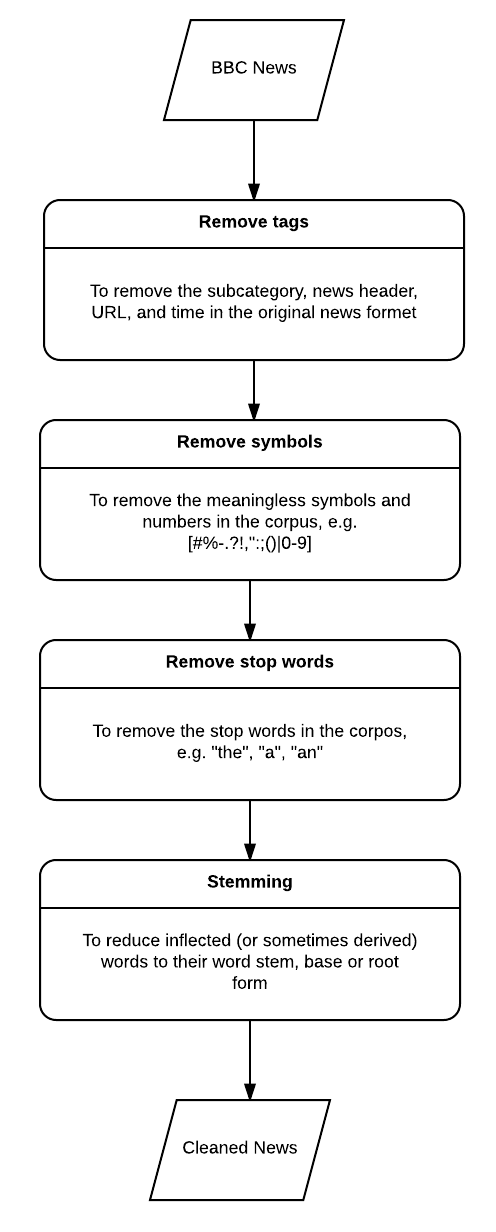
\includegraphics[width=0.5\textwidth]{figures/pipeline.png}
\caption{Preprocessing pipeline for BBC news.}
\label{fig:pipeline}
\end{figure}
\section{Baselines}
\subsection{Topic (LDA) model}

\begin{figure}[h]
\centering
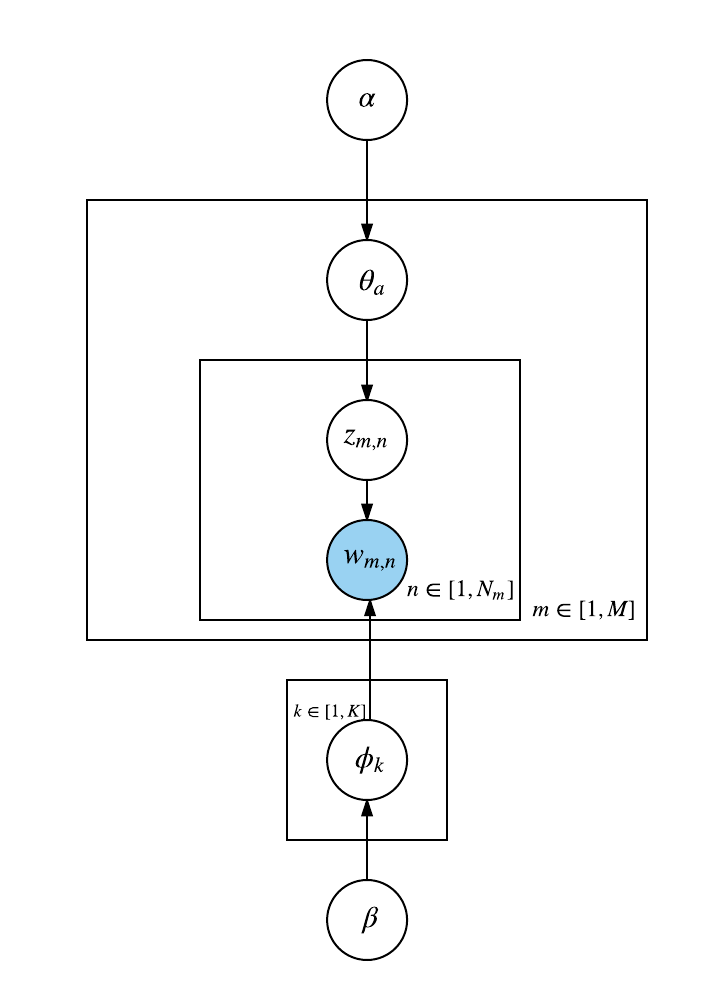
\includegraphics[width=0.6\textwidth]{figures/LDA.png}
\caption{Graphical representation of LDA topic model.}
\label{fig:atot}
\end{figure}

\subsection{Author-Topic model} \label{Author-Topic model}

 
\begin{eqnarray*} \label{eq:at}
\boldsymbol{\Theta}_a | \boldsymbol{\alpha} & \sim & \text{Dirichlet}(\boldsymbol{\alpha})\\
\boldsymbol{\Phi_{k}} | \boldsymbol{\beta} & \sim & \text{Dirichlet}(\boldsymbol{\beta})\\
z_{m,n} | \boldsymbol{\Theta_{x_{m,n}}} & \sim & \text{Multinomial}(\boldsymbol{\Theta_{x_{m,n}}})\\
w_{m,n} | \boldsymbol{\Phi_{z_{m,n}}} & \sim & \text{Multinomial}(\boldsymbol{\Phi_{z_{m,n}}})\\
x_{m,n} | A_m & \sim & \text{Multinomial}(1/A_m)\\

\end{eqnarray*}


\begin{figure}[h]
\centering
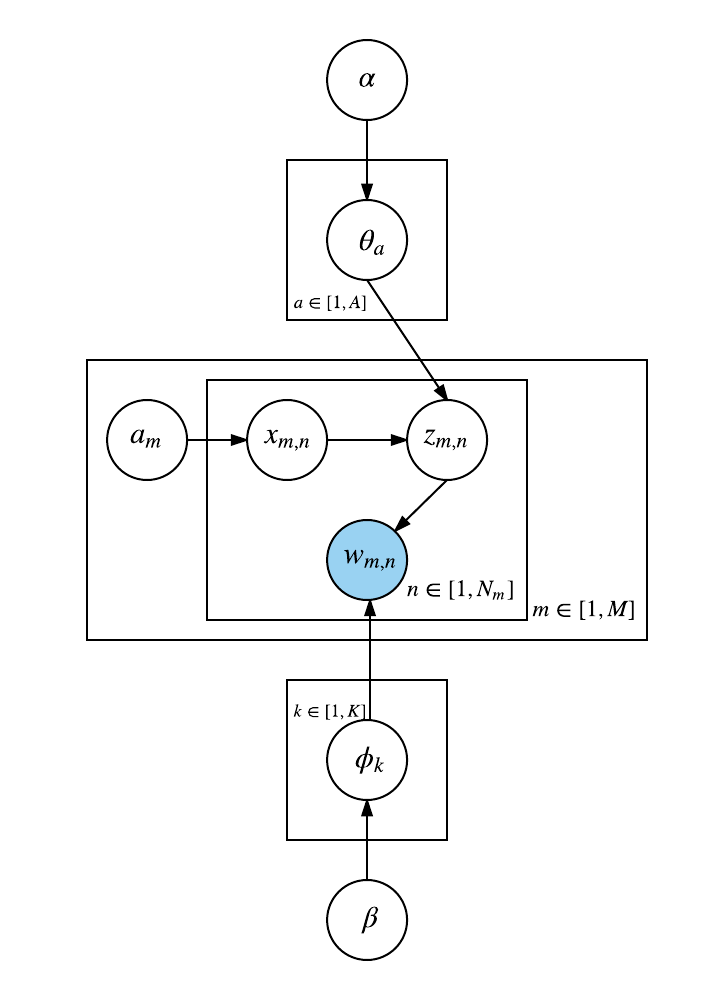
\includegraphics[width=0.6\textwidth]{figures/AT.png}
\caption{Graphical representation of Author-Topic model.}
\label{fig:atot}
\end{figure}

\subsection{Dynamic Topic model}

\begin{figure}[h]
\centering
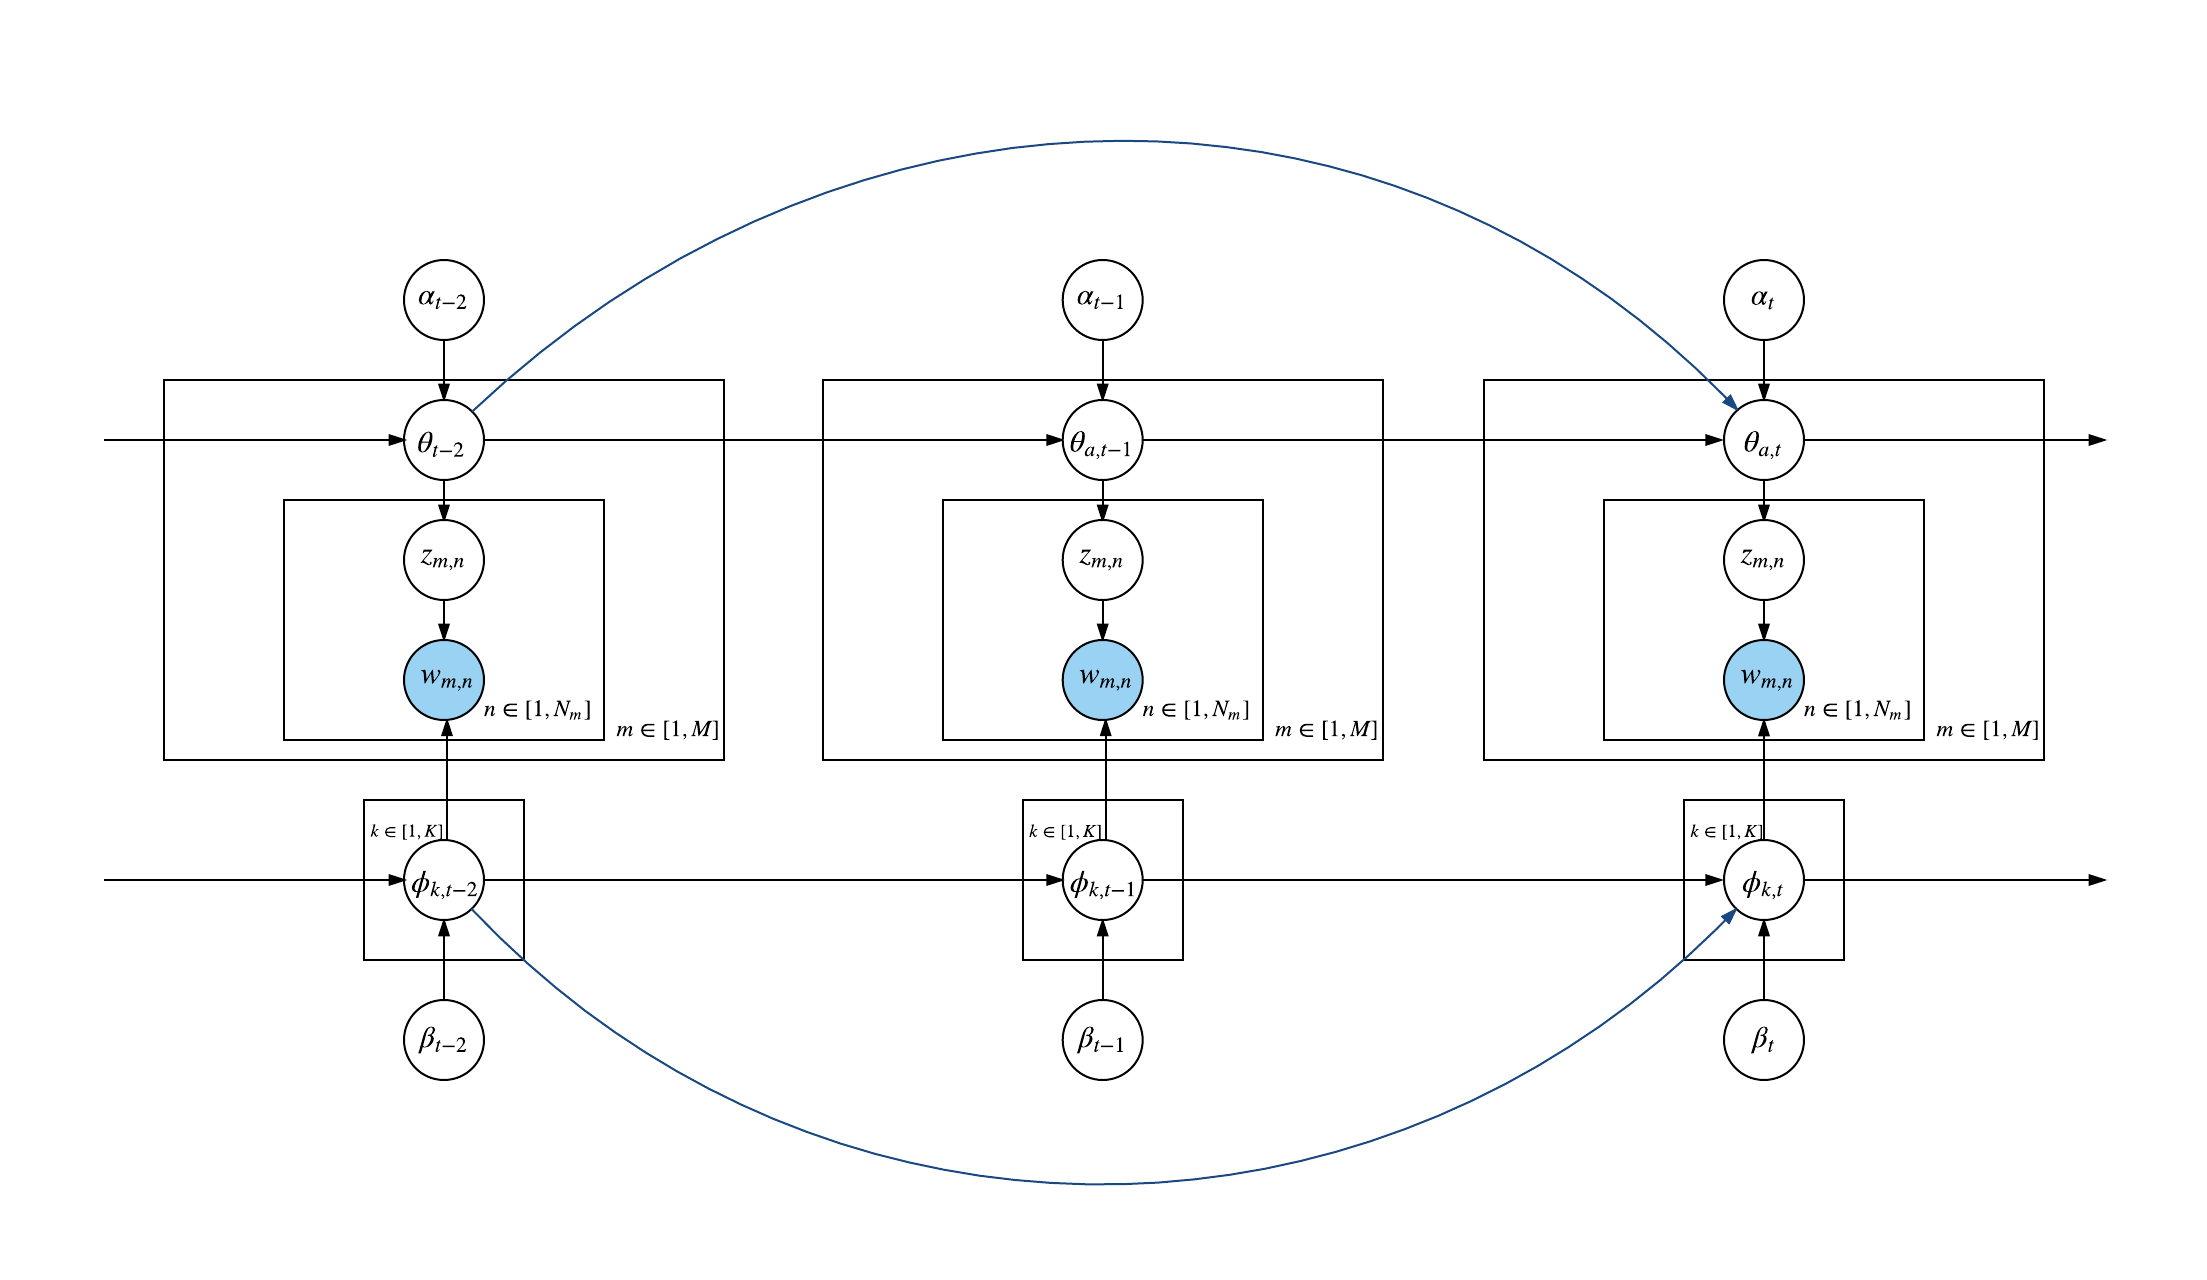
\includegraphics[width=\textwidth]{figures/TOT.png}
\caption{Graphical representation of Dynamic Topic model.}
\label{fig:atot}
\end{figure}

\section{Evaluation Metrics}
Perplexity is a common  evaluation criterion for the performance of Gibbs sampler, namely when the performance of a model trained with sampling begins to level out, which means the Markov chain reaches its convergence. In our experiment we use perpelexity to assess when the performance of our model begins to stabilize, showing how good our classification of topics and authors are.
The perplexity of a set of words is defined as the exponential of negative normalized predictive likelihood under this model, the perplexity of a news $m$
with length $N_m$ containing the set of the words $\boldsymbol{w_m}$ is conditioned on the known authors $\boldsymbol{a}$ of this news and also the time-frame $t$ since ours is a dynamic model. 

\begin{equation}\label{eq:perplexity0}
\mathcal L (\boldsymbol w)
    = \log p(\boldsymbol w | \boldsymbol a, t)
    = \sum_m \log p(\boldsymbol w_m | \boldsymbol a, t)
\end{equation}

Further, in our case we only have one author for each news, therefore if can be deducted as,
\begin{equation}\label{eq:perplexity0}
\begin{split}
\sum_m \log p(\boldsymbol w_m | \boldsymbol a, t)&=\sum_{t=1}^T\sum_{m=1}^{M_t} \log p(\boldsymbol w_m | \boldsymbol a, t)\displaybreak[1]\\
&=\sum_{m=1}^M \sum_{n=1}^{N_M}\log p(w | a_m, t)\displaybreak[1]\\
&=\sum_{m=1}^M \sum_{n=1}^{N_M}\log \sum_{k=1}^K p(w | t,k,a_m)p(k | t,a_m)\displaybreak[1]\\
\end{split}
\end{equation}

 In ~\ref{eq:perplexity0} it shows the log-likelihood of a set of news which contain the word sets $\boldsymbol{w}$ given the author of the news and the time if it is dynamic model. Likelihood of news can be used to compare models, higher likelihood implies a better model. Then the perplexity is traditionally used to measure the topic model, which is derived from \ref{eq:perplexity0}, as follows,
 \begin{equation}\label{eq:perplexity1}
 \text{perplexity}(\boldsymbol w) =
        \exp \left\{
        - \frac{\mathcal L(\boldsymbol w)}{\sum_{m=1}^M{N_m}}
        \right\}
\end{equation}
 
%\begin{equation}\label{eq:perplexity1}
%\text{Perplexity}(w_{m,n}|a_m) = exp(-\frac{\text{log} %p(w_{m,n}|a_m,M^\text{train})}{N_m})
%\end{equation}

From ~\ref{eq:perplexity1} we then drop the dependency of the hyperparameters $\alpha$ and $\beta$, we then approximate the integrals over $\boldsymbol{\theta}$ and $\boldsymbol{\phi}$ using the point estimation. By averaging over multiple samples we can finally obtain the probability $p(w_{m,n}|a_m,M^\text{train})$ as in formula ~\ref{eq:perplexity2},
\begin{equation}\label{eq:perplexity2}
p(w_{m,n}|a_m,M^\text{train}) \approx \frac{1}{S} \sum_{s=1}^{S}\prod_{n=1}^{N_m}[\frac{1}{A_m}\sum_{k}\theta_{a_m,k}\phi_{w_{m,n},k}|\boldsymbol{x^s},\boldsymbol{z^s},M^\text{train},\alpha,\beta]
\end{equation}

in which $A_m = 1$. 